\subsection{Introduction}

\begin{frame}{LoRa}
\framesubtitle{Introduction}
\begin{center}
\scalebox{0.8}{%
\begin{tikzpicture}[auto,node distance=1.2cm]
  \tikzstyle{comment}=[ right=2pt, font=\small, fill=white, text=black, draw=black, ]
  \tikzstyle{every state}=[rectangle,thick,draw=black,fill=gray!20,text=black, minimum width= 6cm, minimum height= 1.00cm ]
  \tikzstyle{smallstate}=[rectangle,thick,draw=black!80,fill=gray!10,text=black, minimum width= 6cm, minimum height= 0.25cm ]
  \tikzstyle{innerstate}=[rectangle,thick,draw=black,fill=gray!10,text=black, minimum width= 4cm, minimum height= 1.00cm ]

  \node[state,color=gray!40,fill=gray!20] at (0, 0) (A)            { Application Layer };
  \node[state,color=gray!40,fill=gray!20]         (E) [below of=A] { Network Layer };
  \node[state,color=gray!40,fill=gray!20]         (F) [below of=E] { Data Link Layer (MAC) };
  \node[state]         (G) [below of=F]                            { LoRa };

  \node[comment]       at (G.north west) {Physical Layer};
\end{tikzpicture}
}
\end{center}

\end{frame}

\begin{frame}{LoRa}
\framesubtitle{Radio Fréquence}
\makebox[\linewidth]{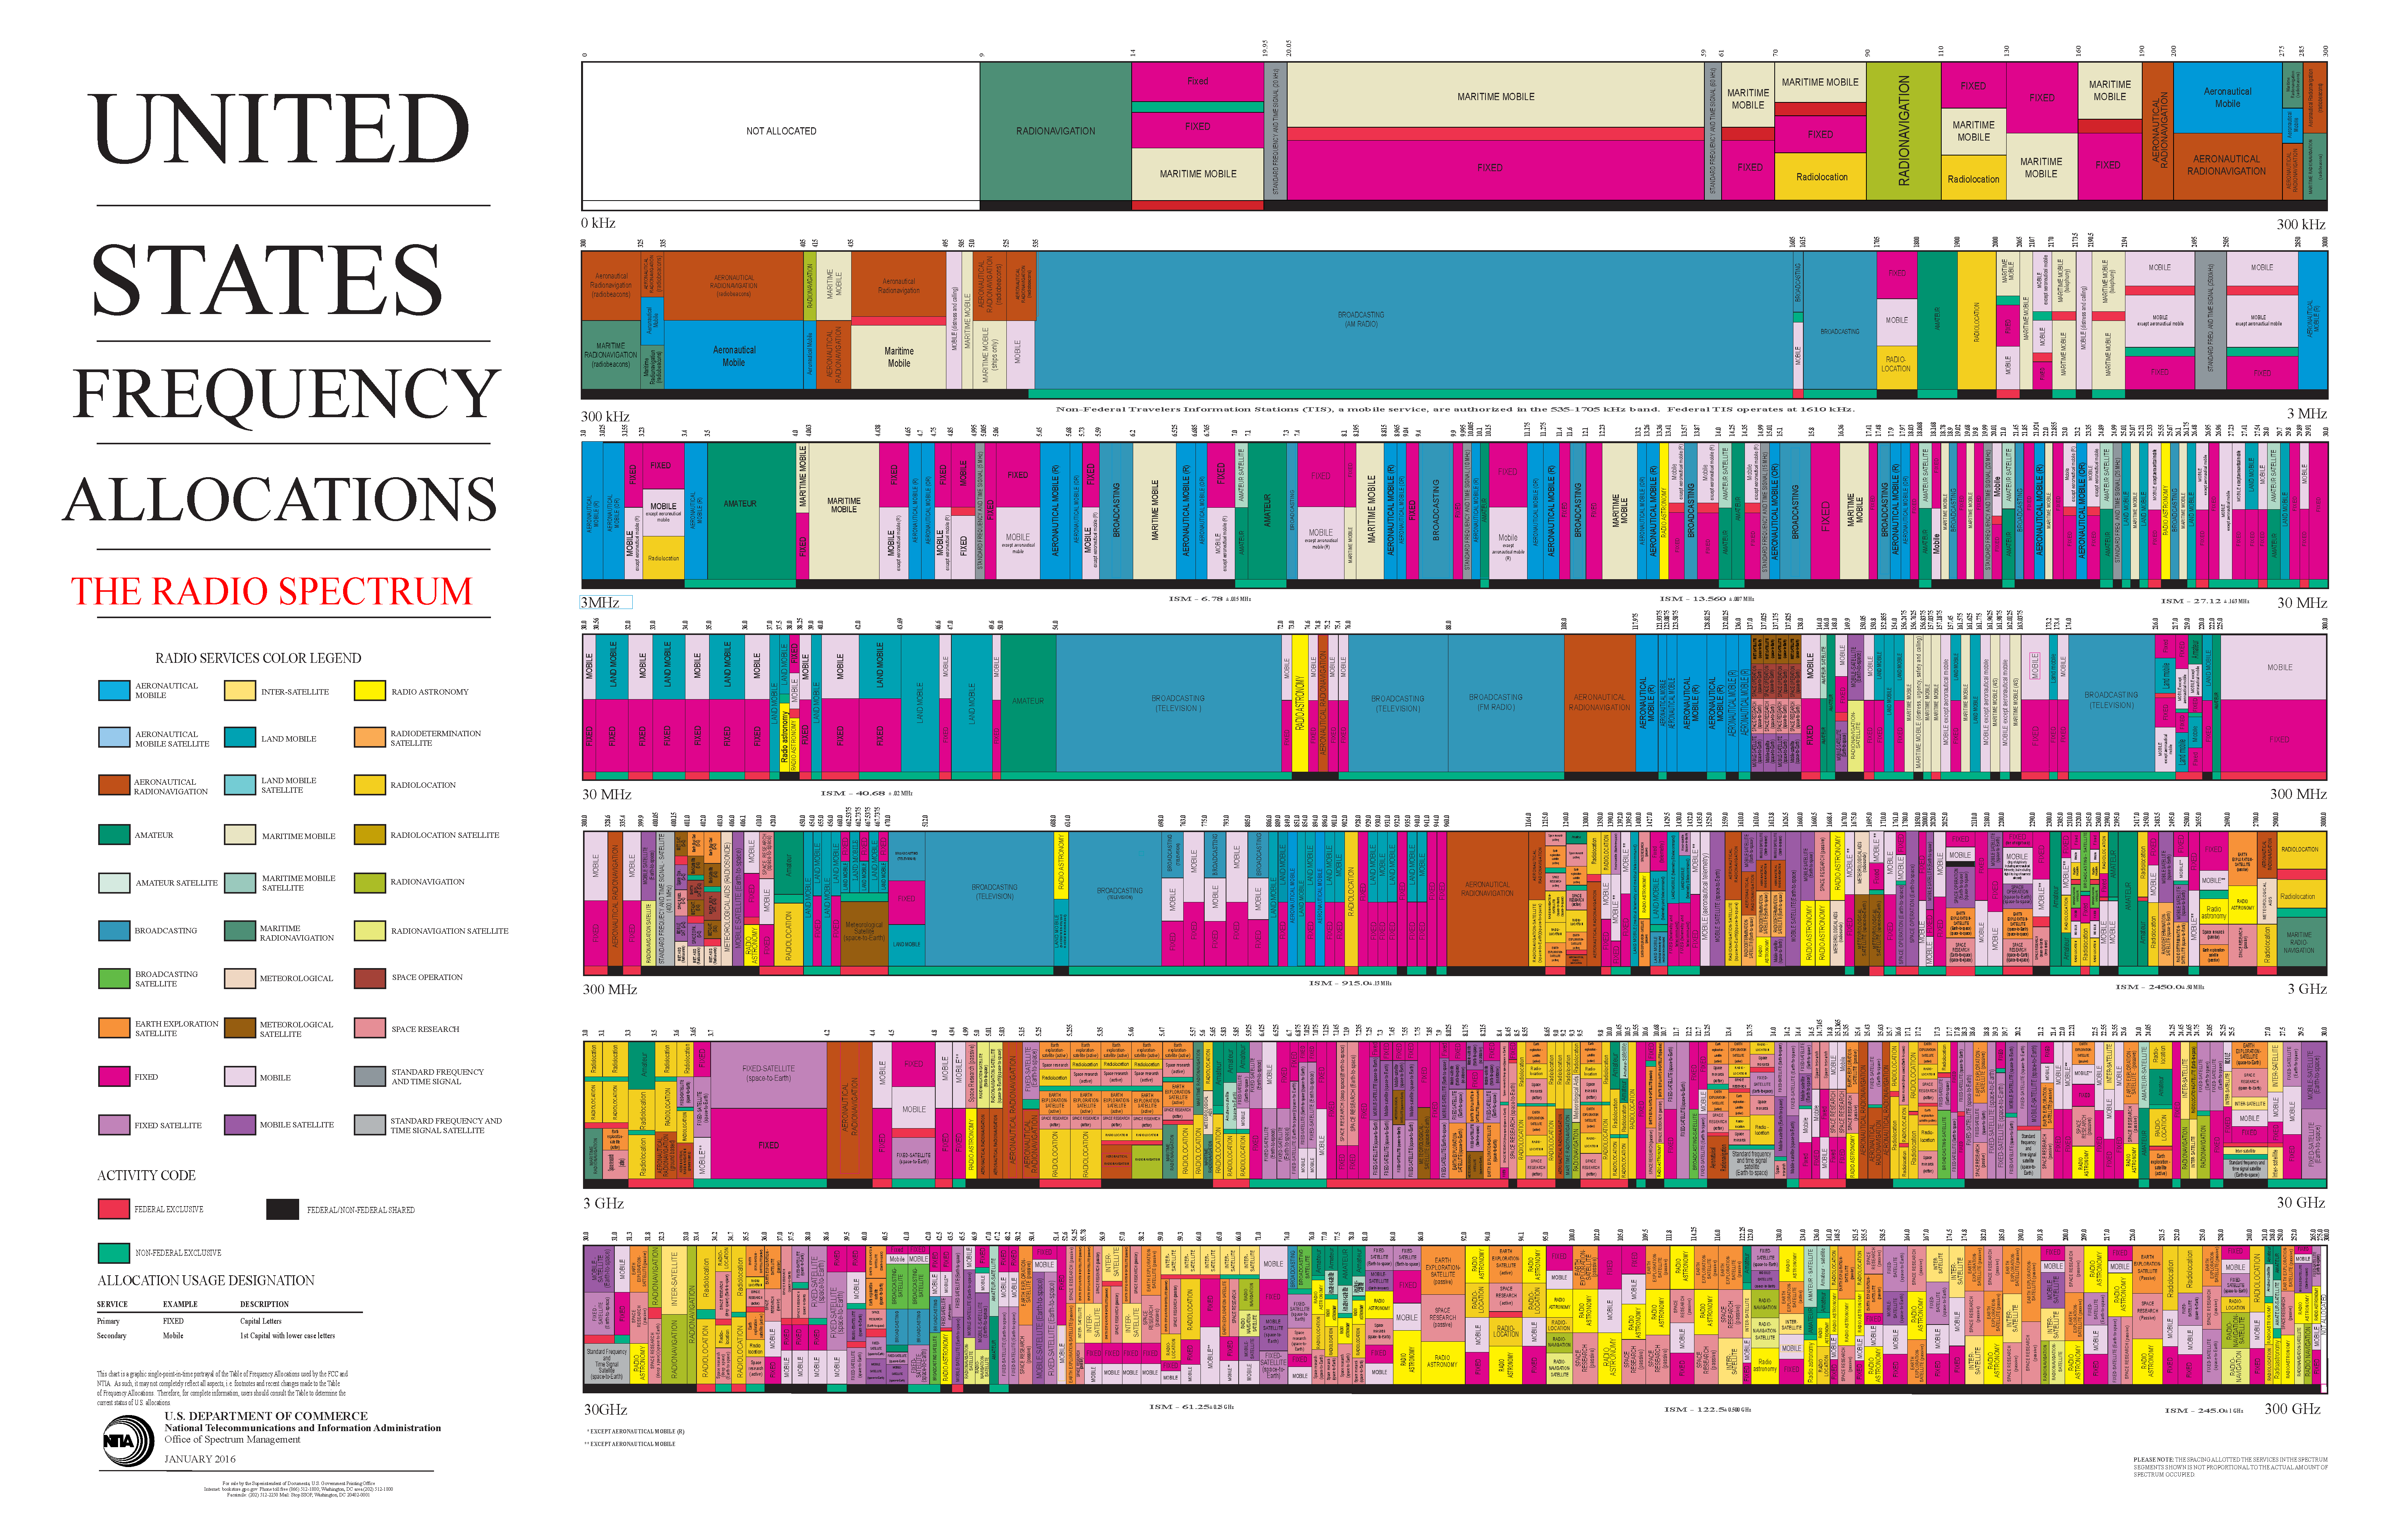
\includegraphics[page=1,width=\paperwidth]{presentation.tex/fig/frequencychart.pdf}}
\end{frame}

\begin{frame}{LoRa}
\framesubtitle{Modulation}
\begin{block}{}
{
Comment transmettre de l'information en utilisant une radio ?
}
\end{block}
\vspace{0.5cm}
\makebox[\linewidth]{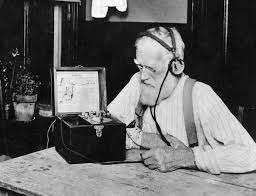
\includegraphics[page=1,width=0.4\paperwidth]{presentation.tex/fig/broadcasting.jpg}}
\end{frame}


\begin{frame}{LoRa}
\framesubtitle{Modulation}
\begin{columns}
\begin{column}{0.5\textwidth}
\begin{itemize}
  \item Signal Analogique
  \begin{itemize}
    \item Voix
    \item Musique
    \item Walkie-talkie
    \item ...
  \end{itemize}
  \item Modulation Analogique
  \begin{itemize}
    \only<1->{\item Modulation de l'amplitude}
    \only<2->{\item Modulation de la frequence}
  \end{itemize}
\end{itemize}  
\end{column}
\begin{column}{0.5\textwidth}
\begin{center}
\scalebox{0.6}{%
\begin{tikzpicture}[samples=1000, domain=0:10*pi]
\begin{axis}[
  width=11cm, height=3.5cm,
  xtick=\empty,
  ytick=\empty,
  xlabel={\large $t$},
  ylabel={\large $x(t)$},
  xmin=0, xmax=11,
  ymin=-3, ymax=5,
  axis lines = middle,
  very thick,
  trig format = rad
]
  \addplot [no markers, smooth, thick] {2.5 + 2*sin(2*pi*0.25*x)};
\end{axis}
  
\begin{axis}[
  at={(0, -2.25cm)},
  width=11cm, height=3.5cm,
  xtick=\empty,
  ytick=\empty,
  xlabel={\large $t$},
  ylabel={\textcolor{blue!60}{carrier wave}},
  xmin=0, xmax=11,
  ymin=-3, ymax=5,
  axis lines = middle,
  very thick,
  trig format = rad
]
  \addplot [no markers, smooth, blue!60, very thick] {2*sin(6*pi*x)};
\end{axis}
  
\only<1>{
\begin{axis}[
  at={(0, -4.5cm)},
  width=11cm, height=3.5cm,
  xtick=\empty,
  ytick=\empty,
  xlabel={\large $t$},
  ylabel={\textcolor{red!60}{AM wave}},
  xmin=0, xmax=11,
  ymin=-3, ymax=5,
  axis lines = middle,
  very thick,
  trig format = rad
]
\addplot expression [no markers, smooth, red!60, very thick] {(2.5 + sin(0.5*pi*x)) * sin(6*pi*x)};
\end{axis}
}

\only<2>{
\begin{axis}[
  at={(0, -4.5cm)},
  width=11cm, height=3.5cm,
  xtick=\empty,
  ytick=\empty,
  xlabel={\large $t$},
  ylabel={\textcolor{green!30!black}{FM wave}},
  xmin=0, xmax=11,
  ymin=-3, ymax=5,
  axis lines = middle,
  very thick,
  trig format = rad
]
  \addplot expression [no markers, smooth, green!30!black, very thick] {2*sin(2*pi*3*x - 8*cos(2*pi*0.25*x))};
\end{axis}
}
\end{tikzpicture}
}
\end{center}

\end{column}
\end{columns}


\end{frame}

\begin{frame}{LoRa}
\framesubtitle{Modulation Digitale}

\begin{block}{}
{
Comment transmettre de l'information numerique avec une radio ?
}
\end{block}
\vspace{0.5cm}
\makebox[\linewidth]{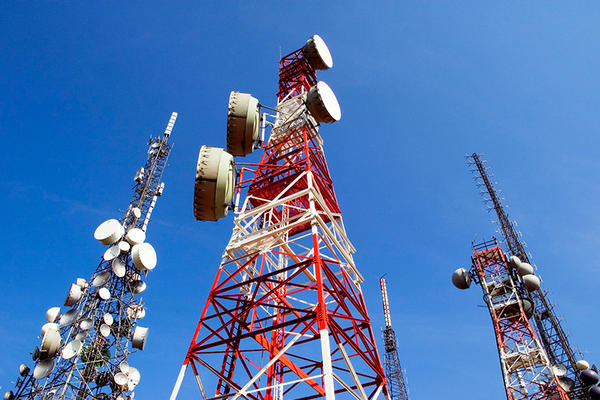
\includegraphics[page=1,width=0.4\paperwidth]{presentation.tex/fig/gsm.jpg}}
\end{frame}

\begin{frame}{LoRa}
\framesubtitle{Modulation Digitale}

\begin{columns}
\begin{column}{0.5\textwidth}
\begin{itemize}
  \item Fréquence
  \item Phase
  \item On/Off
  \item Pulse
\end{itemize}  
\end{column}
\begin{column}{0.5\textwidth}
\begin{center}
\scalebox{0.6}{%
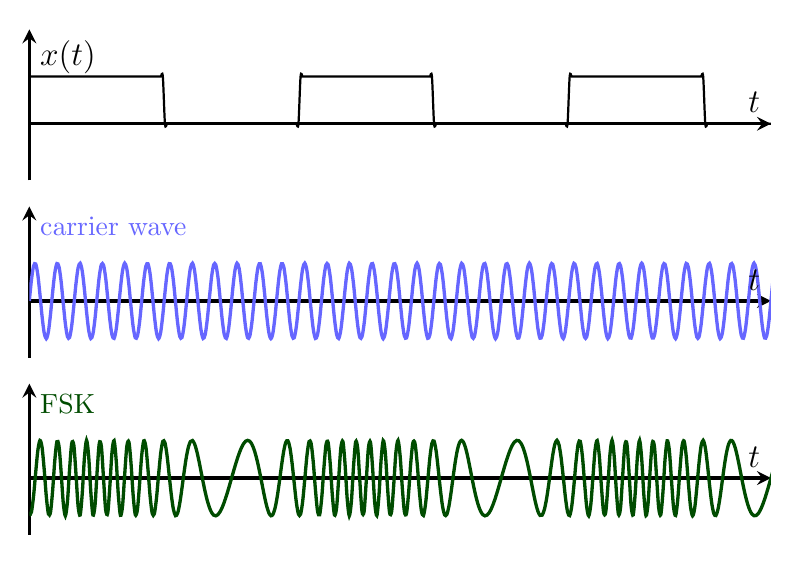
\begin{tikzpicture}[samples=1000, domain=0:10*pi]
\begin{axis}[
  width=11cm, height=3.5cm,
  xtick=\empty,
  ytick=\empty,
  xlabel={\large $t$},
  ylabel={\large $x(t)$},
  xmin=0, xmax=11,
  ymin=-3, ymax=5,
  axis lines = middle,
  very thick,
  trig format = rad
]
  \addplot [no markers, smooth, thick] {2.5 + 2.5*floor(sin(2*pi*0.25*x))};
\end{axis}
  
\begin{axis}[
  at={(0, -2.25cm)},
  width=11cm, height=3.5cm,
  xtick=\empty,
  ytick=\empty,
  xlabel={\large $t$},
  ylabel={\textcolor{blue!60}{carrier wave}},
  xmin=0, xmax=11,
  ymin=-3, ymax=5,
  axis lines = middle,
  very thick,
  trig format = rad
]
  \addplot [no markers, smooth, blue!60, very thick] {2*sin(6*pi*x)};
\end{axis}
  
\begin{axis}[
  at={(0, -4.5cm)},
  width=11cm, height=3.5cm,
  xtick=\empty,
  ytick=\empty,
  xlabel={\large $t$},
  ylabel={\textcolor{green!30!black}{FSK}},
  xmin=0, xmax=11,
  ymin=-3, ymax=5,
  axis lines = middle,
  very thick,
  trig format = rad
]
  \addplot expression [no markers, smooth, green!30!black, very thick] {2*sin(2*pi*3*x - 8*cos(2*pi*0.25*x))};
\end{axis}
\end{tikzpicture}
}
\end{center}

\end{column}
\end{columns}
\end{frame}

\begin{frame}{LoRa}
\framesubtitle{Qu'est-ce que LoRa ?}
\begin{columns}
  \begin{column}{0.6\textwidth}
    
  \begin{itemize}
    \item Une methode de modulation propriétaire
    \begin{itemize}
      \item Creer par Semtech
      \item Grenoble, France
    \end{itemize}
    \item Transmet sur la bande ISM
    \begin{itemize}
      \item 868MHz
    \end{itemize}
    \item Longue distance de transmission
    \item Basse consommation
    \item Différent paramêtres influence la communication
  \end{itemize}
  \end{column}
  \begin{column}{0.4\textwidth}
    \makebox[\linewidth]{
\includegraphics[page=1,width=0.45\paperwidth]{presentation.tex/fig/lora.png}}
  \end{column}
\end{columns}
\end{frame}

\begin{frame}{LoRa}
\framesubtitle{Chirp Spread Spectrum}
\begin{block}
Information transmit à l'aide de 'chirp'
\end{block}
\begin{columns}
  \begin{column}{0.5\textwidth}
    \begin{center}
\scalebox{0.8}{
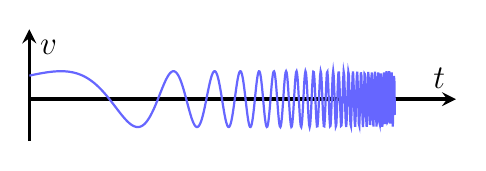
\begin{tikzpicture}
\begin{axis}[
  samples=700,
  domain=0:3*pi,
  width=7cm, height=3cm,
  xtick=\empty,
  ytick=\empty,
  xlabel={\large $t$},
  ylabel={\large $v$},
  xmin=0, xmax=11,
  ymin=-3, ymax=5,
  axis lines = middle,
  very thick,
  trig format = rad
]
\addplot[thick, blue!60]plot (\x, {2*sin(pow(2,(0.8*\x)))});
\end{axis}
\end{tikzpicture}
}
\end{center}

  \end{column}
  \begin{column}{0.5\textwidth}
    \begin{center}
      \makebox[\linewidth]{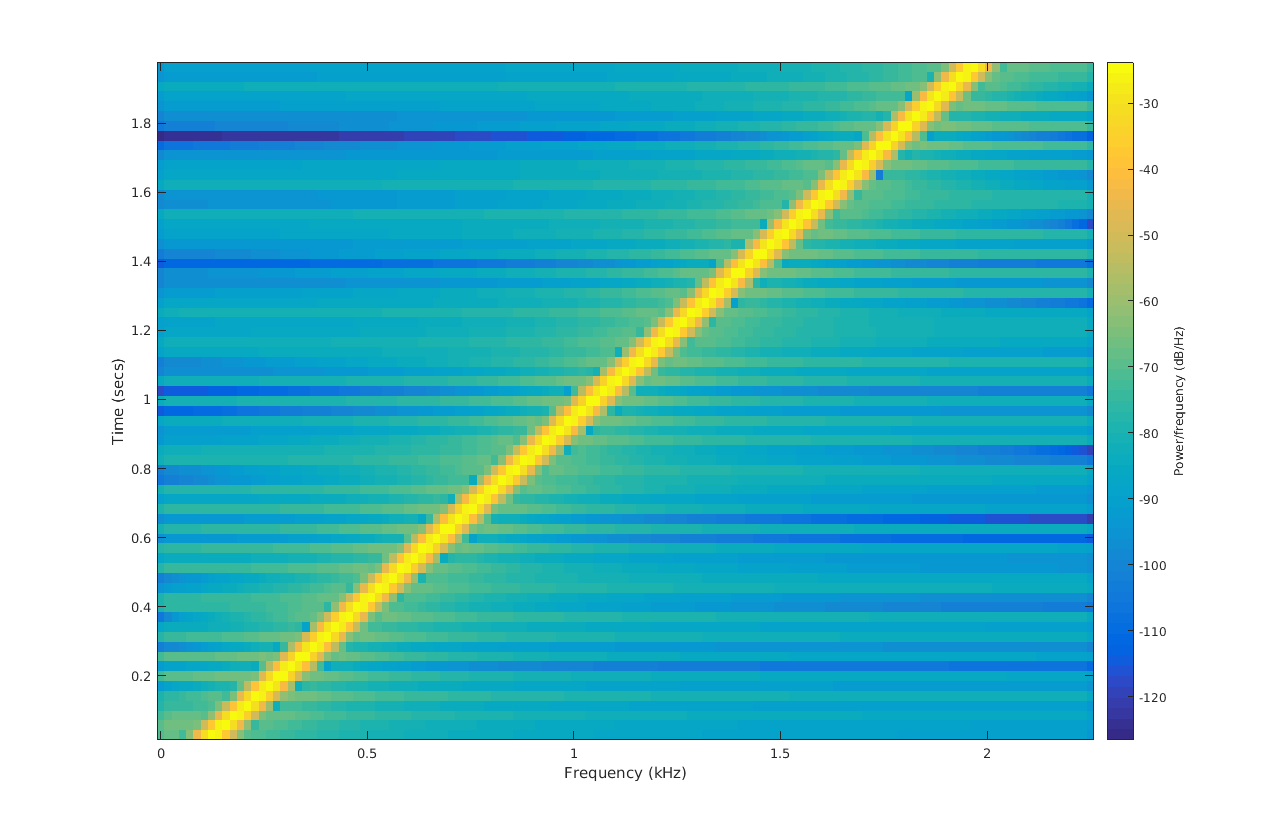
\includegraphics[page=1,width=0.55\paperwidth]{presentation.tex/fig/upchirp.png}}
    \end{center}
  \end{column}
\end{columns}
\end{frame}

\begin{frame}{LoRa}
\framesubtitle{Chirp Spread Spectrum}
\begin{columns}
  \begin{column}{0.5\textwidth}
    \begin{itemize}
      \item Chaque 'chirp' est modulé pour transmettre de l'information
      \item La modulation est propriétaire
    \end{itemize}
  \end{column}
  \begin{column}{0.5\textwidth}
    \begin{center}
      \makebox[\linewidth]{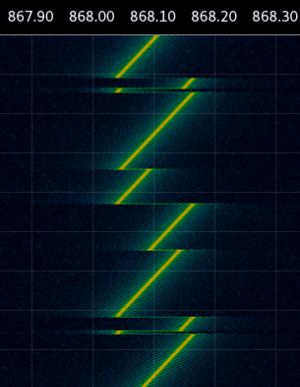
\includegraphics[page=1,width=0.40\paperwidth]{presentation.tex/fig/loraspectrum.png}}
    \end{center}
  \end{column}
\end{columns}
\end{frame}

\begin{frame}{LoRa}
\framesubtitle{Bandwidth}
\begin{columns}
\begin{column}{0.5\textwidth}
    
\begin{itemize}
  \item 500, 250, 125 kHz
  \item $\nearrow$ bande passante $=$ $\nearrow$ bruit
  \item $\nearrow$ bande passante $=$ $\nearrow$ portée
  \item $\nearrow$ bande passante $=$ $\searrow$ débit
\end{itemize}
\end{column}
\begin{column}{0.5\textwidth}
  \begin{center}
\scalebox{0.70}{%
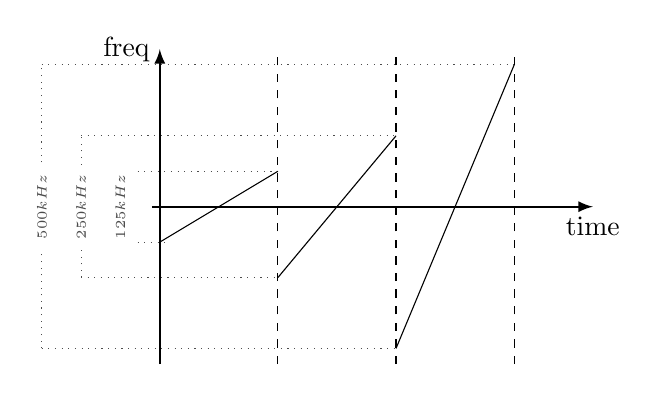
\begin{tikzpicture}[
  arr/.style={help lines,black!70,<->},
]
  \draw[thick,-latex] (0,-2) -- (0,2)node[left] {freq};
  \draw[thick,-latex] (-0.1,0) -- (5.5,0)node[below] {time};
  \draw[dashed] (1.5,-2) -- (1.5,2);
  \draw[dashed] (3.0,-2) -- (3.0,2);
  \draw[dashed] (4.5,-2) -- (4.5,2);

  \draw[dotted,black!70] (-0.45,0.45) -- (1.5,0.45);
  \draw[dotted,black!70] (-0.45,-0.45) -- (0.1,-0.45);
  %
  \draw[dotted,black!70] (-1.0,0.9) -- (3.0,0.9);
  \draw[dotted,black!70] (-1.0,-0.9) -- (1.5,-0.9);
  \draw[dotted,black!70] (-1.0,-0.9) -- (-1.0,0.9);
  %
  \draw[dotted,black!70] (-1.5,1.8) -- (4.5,1.8);
  \draw[dotted,black!70] (-1.5,-1.8) -- (3.0,-1.8);
  \draw[dotted,black!70] (-1.5,-1.8) -- (-1.5,1.8);

  \node[rotate=90, black!70,fill=white] at (-0.5,0) {\tiny $125kHz$};
  \node[rotate=90, black!70,fill=white] at (-1.0,0) {\tiny $250kHz$};
  \node[rotate=90, black!70,fill=white] at (-1.5,0) {\tiny $500kHz$};

  \draw[] (0,-0.45) -- (1.5,0.45);
  \draw[] (1.5,-0.9) -- (3.0,0.9);
  \draw[] (3.0,-1.8) -- (4.5,1.8);

  % \draw[arr] (0.1, -2.2) -- node[fill=white] {$SF7$} (1.4, -2.2);
  % \draw[arr] (1.6, -2.2) -- node[fill=white] {$SF7$} (2.9, -2.2);
  % \draw[arr] (3.1, -2.2) -- node[fill=white] {$SF7$} (4.4, -2.2);
\end{tikzpicture}
}
\end{center}

\end{column}
\end{columns}
\end{frame}

\begin{frame}{LoRa}
\framesubtitle{Spreading Factor (SF)}
\begin{columns}
  \begin{column}{0.4\textwidth}
    \begin{itemize}
      \item Longueur du chirp
      \item Nombre de symbôle encodé par chirp
      \item Orthogonalite des SF
      \begin{itemize}
        \item Communications concurentielles
      \end{itemize}
      \item  $R_{s} = \frac{BW}{2^{SF}}$
      \item $\nearrow$ SF $=$ $\nearrow$ portée
    \end{itemize}
  \end{column}
  \begin{column}{0.6\textwidth}
    \begin{center}
\scalebox{0.6}{%
\begin{tikzpicture}[
  arr/.style={help lines,black!70,<->},
]
  \draw[thick,-latex] (0,-2) -- (0,2)node[left] {frequency};
  \draw[thick,-latex] (-1,0) -- (11.5,0)node[below] {time};
  \draw[dashed] (1.5,-2) -- (1.5,2);
  \draw[dashed] (4.5,-2) -- (4.5,2);
  \draw[dashed] (10.5,-2) -- (10.5,2);
  \draw[] (0,-1.8) -- (1.5,1.8);
  \draw[] (1.5,-1.8) -- (4.5,1.8);
  \draw[] (4.5,-1.8) -- (10.5,1.8);

  \draw[arr] (0.1, -2.2) -- node[fill=white] {$SF7$} (1.4, -2.2);
  \draw[arr] (1.6, -2.2) -- node[fill=white] {$SF8$} (4.4, -2.2);
  \draw[arr] (4.6, -2.2) -- node[fill=white] {$SF9$} (10.4, -2.2);
\end{tikzpicture}
}
\end{center}

  \end{column}
\end{columns}
\end{frame}
